\section{Empirical data}\label{sec:data}
% 
//Intro about section on empirical data = interviews + surveys other people did
% 
\subsection{Interviews}
% 
//Small intro about interview we did and interview guide we developed.
% 
\subsubsection{Interview with Finn Bjerremand}

Early in the process we have contacted Morten Lindbo, press officer of DTL (Danish Transport and Logistics association). He responded with contacts of their technical consultant and test driver - Finn Bjerremand.\par
% 
Interview on 27th of April was taken via Skype call since we were located in different cities.\par
% 
Finn took part in a research project about truck platooning as a test driver. Trucks in platoon were travelling between two cities in Denmark, distance of around 300km.\par
% 
SCANIA trucks were equipped with ACC (Adaptive Cruise Control) that means it was not fully automated platoon. Finn also noticed that experience of driving with ACC in short distance (9-12 meters) platoon was very similar to regular driving. And because truck drivers usually keep very short distance between each other, Finn thinks that truck platooning will make big improvement for safety on the roads. He was excited about user experience for the drivers as platooning will increase comfort and usability.\par
% 
We introduced Finn with our research problem, and asked about his knowledge about forming ad hoc platoons while being on the road. He saw one main problem comparing to platoons that have set route - "who will pay for who?". Finn thinks it will be difficult to make ad hoc platooning beneficial for everyone, as leading car uses much more fuel than others.\par
% 
Platoon in the experiment did not use any V2V communication and was dependant on ACC for longitudinal automation and drivers for steering the wheel. Finn is also aware of fully automated experiments made by VOLVO or SCANIA, he is excited about driving experience where you don't have to do that much and can even take your breaks without stopping. Although Finn thinks that it will take long time until fully automated platooning will be possible not only on highways.\par
% 
It was relaxed and very informal interview. We greatly appreciate time from Finn Bjerremand. Interview has provided us with useful remarks about driving experience in a platoon and some concerns regarding ad hoc platooning.
% 
\subsection{Secondary data}
% 
//Explanation about other empirical data we gathered (like \cite{Shladover2015IndustryPlatooning}), SAFESPOT, COMPANION, etc. and maybe others (presentation Reza gave us on 04/05?).\par
% 
To prove that platooning is not just another technology being developed without a real added value, several projects and researches has been made to obtain the data to prove its benefits (some of them are mentioned in Literature review chapter - \hyperref[sec:SARTRE]{SARTRE}, \hyperref[sec:Companion]{Companion}). As we didn’t have sufficient budget and time to do the whole development of the system and later on to carry out test to get the data, we looked into those projects to find out whether platooning will be beneficial for people. The areas we tried to cover are fuel consumption, drag, latency, and monetising.
% 
\subsubsection{Fuel savings}\label{sec:fuel-savings}
% 
The lower fuel consumption is one of the main benefit of platooning and one of the main reasons why freight companies would adapt this technology. But in order to convince these companies, there must be clear evidence that platooning really saves fuel. In SARTRE \cite{Chan2012ProjectSARTRE} the CFD (Computational Fluid Dynamic) aerodynamic simulations and real life testing have been done to find it out.
%
\subsubsection*{CFD test}
In CFD test 5 vehicles were involved, 2 trucks and 3 cars, the order was leading truck, following truck and 3 following cars. Tests were done with different distance between vehicles starting with 3 meters till 15 meters. Here vehicles were perfectly aligned behind each other. Figure \ref{fig:cx-reduction} shows by how many percent the drag of vehicles has been reduced with different distances between them. It seems like the closer vehicles are, the better as the drag reduction (Cx) is higher. From simulation, the best fuel saving distance is 3-4 meters. However, having vehicles so close to each other causes instabilities and therefore the best distance would be 6-8 meters according to SARTRE project \cite[p. 33]{Chan2012ProjectSARTRE}.\par
% 
\begin{figure}[p]
    \centering
    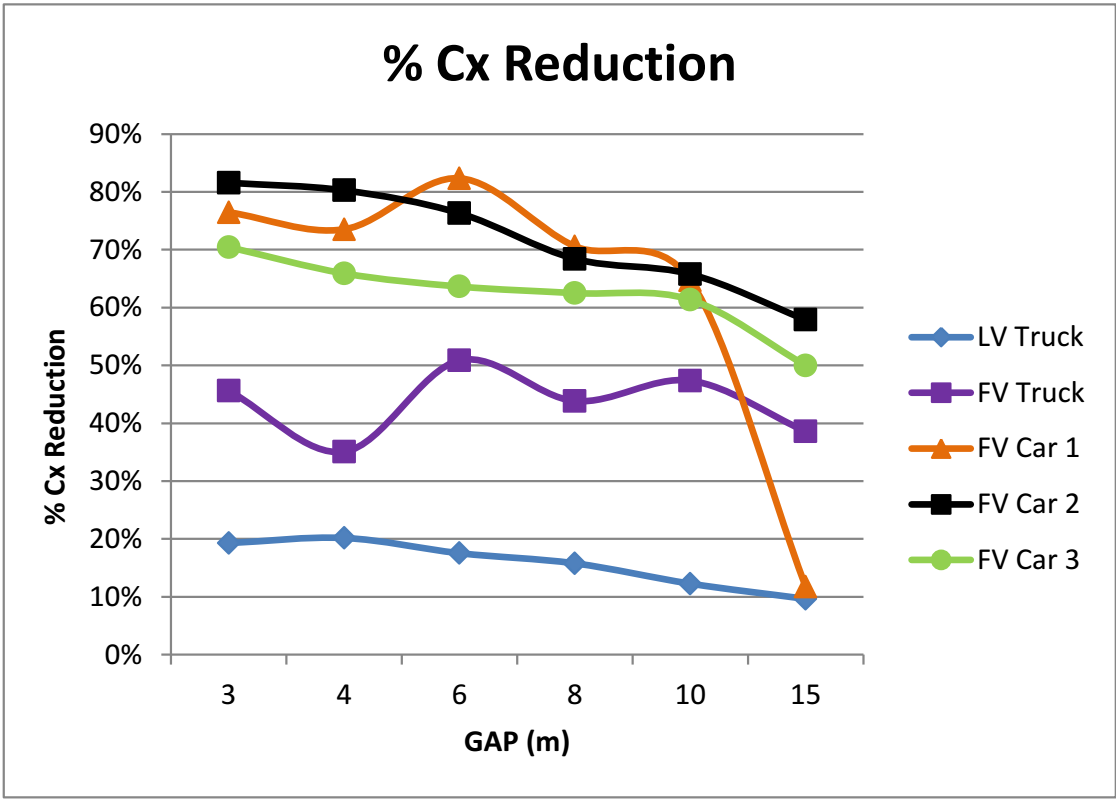
\includegraphics[width=.95\textwidth]{cx-reduction}
    \caption{Drag reduction for platooning vehicles as a function of gap between them. CFD simulation. Taken from \cite{Chan2012ProjectSARTRE}}
    \label{fig:cx-reduction}
\end{figure}
% 
In the test mentioned above the vehicles were perfectly aligned. This however, is very unlikely to happen in real life. Therefore, in the Companion project when making simulation virtually they count with this offset of vehicles and measured difference in drag of 2 truck with different lateral offset, the distance between trucks was 3 meters. The simulated offset was 0.1, 0.25, 0.5 and 1 meter. The Figure \ref{fig:lateral-offset} shows the results of simulations.
% 
\begin{figure}[p]
    \centering
    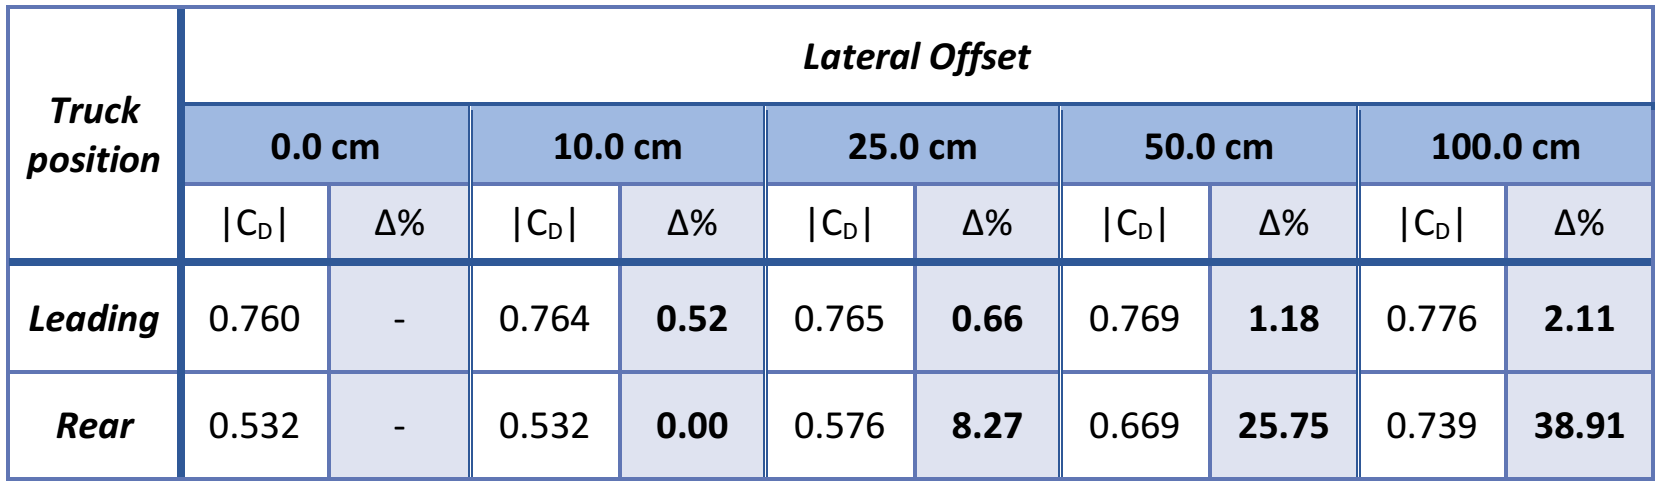
\includegraphics[width=.95\textwidth]{lateral-offset}
    \caption{Difference in drag by lateral offset. CFD simulation. Taken from \cite[p. 19]{Laxhammar2015CooperativeConsumption}}
    \label{fig:lateral-offset}
\end{figure}
% 
As it can be seen in Figure \ref{fig:lateral-offset} small lateral offset of 10 cm does not influence the drag at all, but as the offset is bigger it can be observed that the following truck experiences pretty high values of drag compared to no offset. There is almost 39\% rise in drag when there is 100 cm offset and the drag value of following truck is almost the same as of the leading one. But for leading truck, different offset values did not change much as the maximum drag rise was a bit more than 2\% which is negligible. From this we found that small offset does not have a noticeable impact on the drag but vehicles should be as aligned as possible.\par
%
\begin{figure}[p]
    \centering
    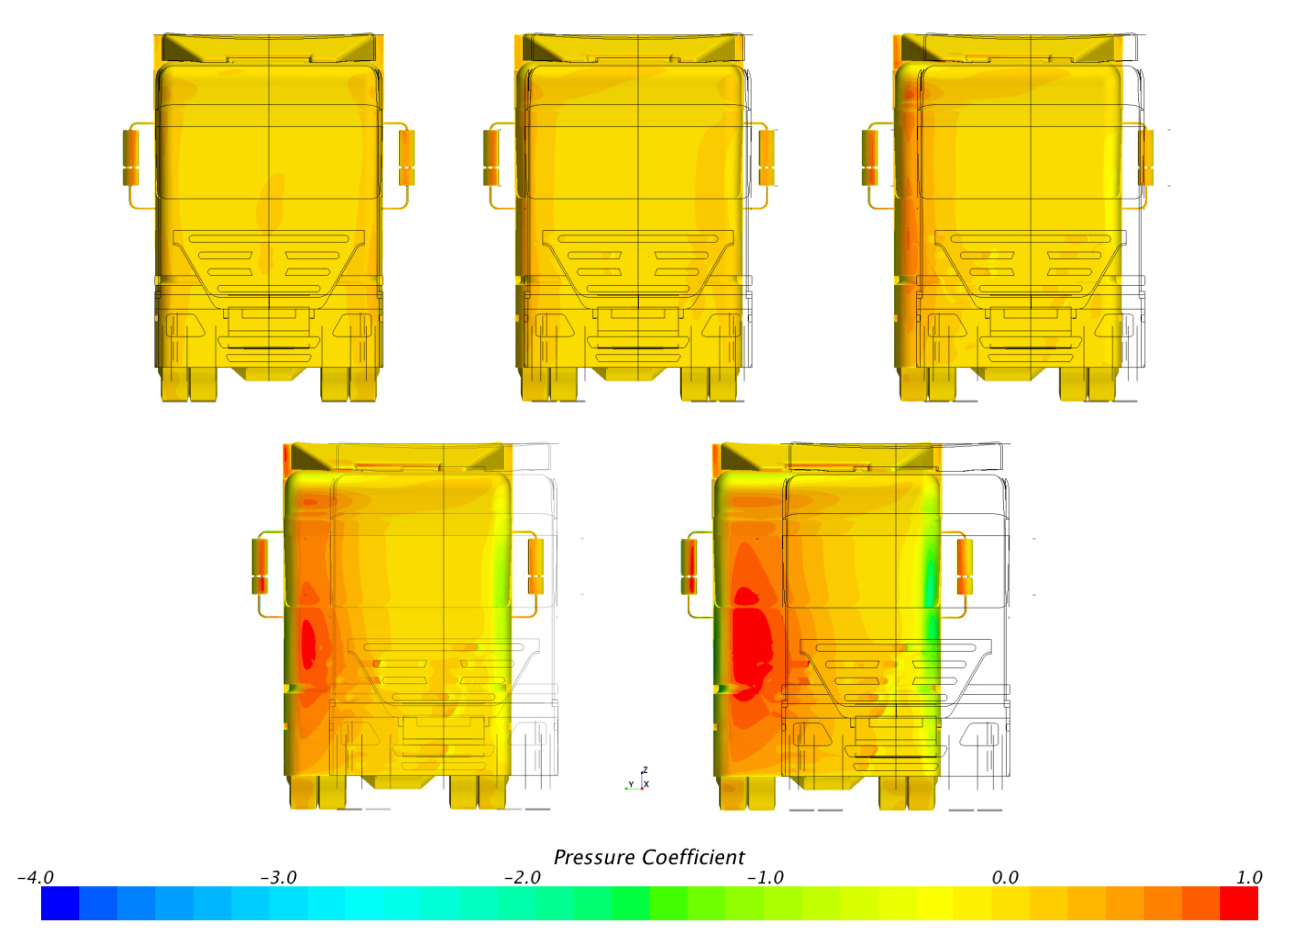
\includegraphics[width=.95\textwidth]{pressure-coef}
    \caption{Pressure on following truck with different offset. CFD simulation. Taken from \cite[p. 19]{Laxhammar2015CooperativeConsumption}}
    \label{fig:pressure-coef}
\end{figure}
% 
% 
\subsubsection*{Real life tests}
In real life tests, a fuel consumption of each vehicle has been first measured separately (not in a platoon) and then in a platoon made up by 2 trucks and 3 cars, the same order as in the CFD simulation. Different distances were tested, starting at 5 meters up to 15 meters. Results are shown in Figure \ref{fig:fuel-savings-full}.\par
% 
As it can be seen in the table, there is a fuel saving effect because of the drag reduction in a platoon in reality as well. The right data could not be measured for cars in distances smaller than 7 meters because of an emergency system which was triggered in cars and made fuel consumption higher. Nonetheless, the graph show that the closer vehicles are the bigger is fuel saving and that also validate that platooning saves fuel.
% 
\begin{figure}[h]
    \centering
    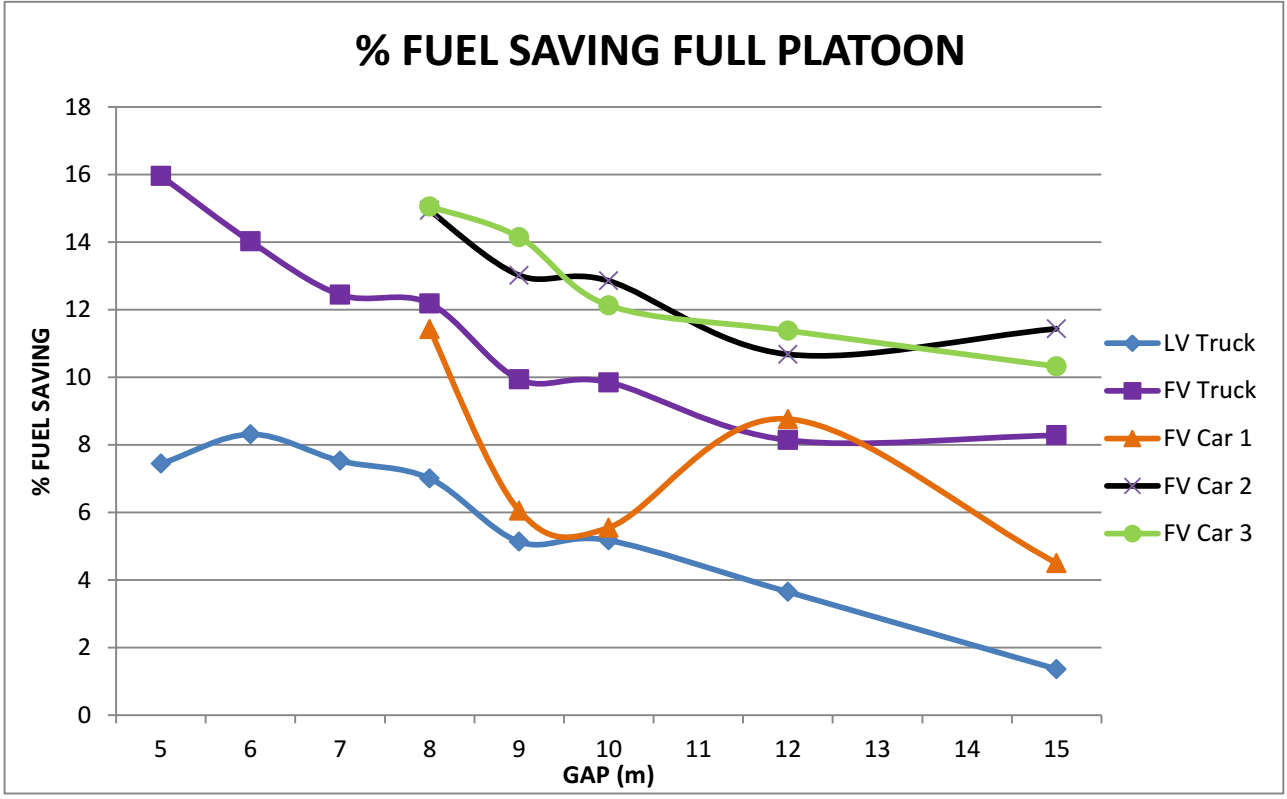
\includegraphics[width=.95\textwidth]{fuel-savings-full}
    \caption{Fuel savings for platooning vehicles. Real-life test. Taken from \cite[p. 36]{Chan2012ProjectSARTRE}.}
    \label{fig:fuel-savings-full}
\end{figure}
% 

% 
\subsubsection{Monetised benefits of platooning}
% 
As shown in the \hyperref[sec:fuel-savings]{previous section}, platooning can save money by lower fuel consumption. But there are higher initial costs and truck will not be platooning 100\% of the time. There comes a question then, whether higher initial costs can be returned over the lifetime of truck and how much can be actually saved. In Companion project, an estimate of the money return has been done, in their deliverable 8.4 \cite{Dr.Hanelt2016CooperativeResults}. To make such a calculation, the estimate price of fuel is needed for year ahead as savings are largely dependent on the price of fuel. Therefore, a forecast for next years had to be done from which the prices will be taken. Table \ref{tab:diesel-costs} shows estimated diesel costs.
% 
\begin{table}[p]
    \centering
    \begin{tabular}{*{10}{|l}| }
        \hline
        \textbf{Year} & 2017 & 2018 & 2019 & 2020 & 2021 & 2022 & 2023 & 2024 & 2025 \\
        \hline
        \textbf{Diesel Price} & 1.18\euro & 1.18\euro & 1.18\euro & 1.20\euro & 1.22\euro & 1.23\euro & 1.25\euro & 1.27\euro & 1.29\euro\\
        \hline
    \end{tabular}
    \caption{Estimated cost of diesel. Taken from \cite[p. 34]{Dr.Hanelt2016CooperativeResults}.}
    \label{tab:diesel-costs}
\end{table}
% 
Other data has been taken also from Companion project deliverable: \textquote[\cite{Dr.Hanelt2016CooperativeResults}]{\textit{The mean age of trucks in Germany is 7.5 years, with 6.2 as the median. Hence, an average use period of seven years per truck is assumed. Relying on previous calculations, a yearly distance of 150,000 km per truck and a fuel consumption of 35 litres per 100 km was assumed. When driving in a platoon of three trucks at a speed of 70 to 80 km/h and a distance of 10 to 20 m between the trucks, the fuel saving potential per truck is 4.99\% on average.}}
Having almost all necessary variables to compute possible investment return, it is needed to choose the commerce year of platooning because of fuel prices. Year 2019 was chosen. Then the last very important think needs to be set and that is the amount of time of which a truck will be platooning, because it will not be doing so always. Four different platooning rates has been chosen: 90\%, 70\%, 50\% and 30\%.\par
% 
\begin{table}[p]
    \centering
    \begin{tabular}{*{3}{|l}|}
        \hline
        \textbf{Platooning rate} & \textbf{Accumulated} & \textbf{Average (p.a.)}\\
        \hline
        \textbf{90\%} & 13,711.72\euro & 1,958.82\euro\\
        \hline
        \textbf{70\%} & 9,186.90\euro & 1,312.41\euro\\
        \hline
        \textbf{50\%} & 4,662.07\euro & 666.01\euro\\
        \hline
        \textbf{30\%} & 137.24\euro & 19.61\euro\\
        \hline
    \end{tabular}
    \caption{Money saved over the lifespan of truck with different platooning rate. Accumulated amount is already lower by initial costs (driving license, truck technology, annual fee, etc.). Accumulated amount is pure saving. Taken from \cite[p.34]{Dr.Hanelt2016CooperativeResults}}
    \label{tab:truck-lifespan}
\end{table}
% 
From the table \ref{tab:truck-lifespan}, it can be seen that even with a low platooning rate of 30\% the higher initial costs will be returned and moreover some small amount of money potentially earned. It is assumed that truck will be platooning more and therefore, this technology should be saving costs to company beside other benefits.
% 
\subsubsection{Latency}
Latency is crucial when it comes to safety in platooning, because if message sent over V2V from leading vehicle to following vehicle fails to arrive on time, it may result in crash. In the SARTRE project (\cite{Chan2012ProjectSARTRE}) they made a test of latency between Back office and Organisation assistant. Back office lies on the server and Organisation assistant is in the vehicle. It communicates with GPS and is sending vehicles’ GPS position to Back office through GSM/UMTS (V2I). Although these are not technologies we are using in V2V it is interesting to see how the latency differs in lower and higher traffic. The test was done on the road in the city as well as outside and in following times: 15:00-16:00 and 18:40–19:30.\par
% 
It can be observed that in the second case, the latency is higher due to the bigger traffic. This reminds us to bear in mind that the bigger the traffic is the bigger the latency and according to that some safety requirements must be set as well (for example: When the latency is higher than X milliseconds, minimum distance between vehicles must be Y meters). Nonetheless the latency should be kept as low as possible, because when using V2V to transmit data the latency may be a difference between safe stop of vehicle and crash.
% 
\begin{figure}[p]
    \centering
    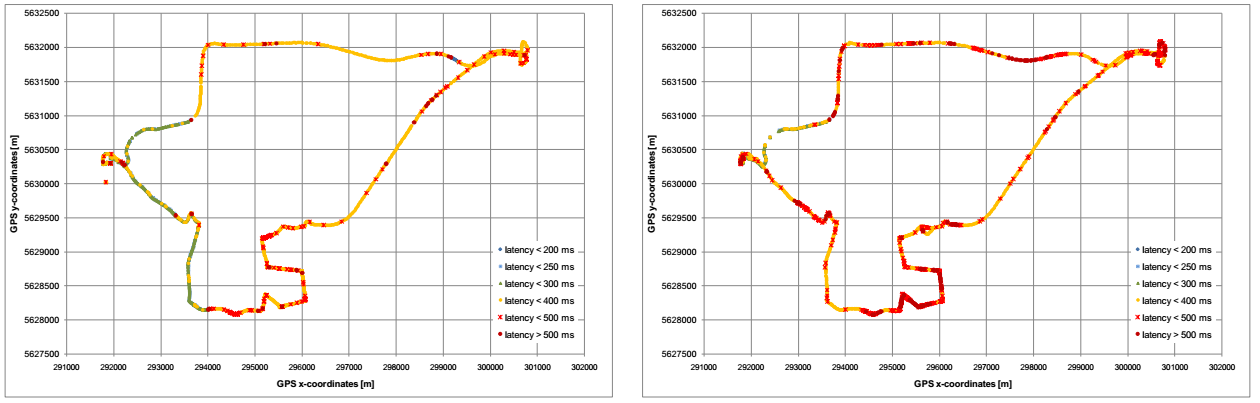
\includegraphics[width=.95\textwidth]{latency}
    \caption{Latency during testing in different day-times: Left 15:00-16:00, right 18:40-19:30. Taken from \cite[p. 24]{Chan2012ProjectSARTRE}}
    \label{fig:latency}
\end{figure}
% 
% 
//Views of Industry on the platooning - little more to be written here.